\chapter{Superfícies, adsorção e catálise heterogênea}\label{ch:b3:surfaces-catalysis}

Debaixo de um carro, dentro de uma lata de aço, há uma colmeia cerâmica cujos
milhares de canais são revestidos por um óxido poroso que contém alguns gramas de
platina, paládio e ródio. Em uma fração de segundo, os gases de escapamento que a
atravessam perdem a maior parte de seu monóxido de carbono, de seus hidrocarbonetos
não queimados e de seus óxidos de nitrogênio. Nada acontece no gás: cada uma dessas
reações ocorre na superfície das partículas metálicas, de alguns nanômetros de
diâmetro. A maior parte da indústria química funciona da mesma maneira, da amônia
dos fertilizantes ao craqueamento do petróleo. Este capítulo descreve como as
moléculas se fixam às superfícies, que parte de uma superfície elas cobrem, como
ocorrem as reações de superfície e como um catalisador sólido é preparado, medido
e observado.

\begin{recall}
O volume do 1.º ano definiu os catalisadores e a diferença entre catálise
homogênea e heterogênea, e descreveu o empacotamento cúbico de faces centradas dos
metais. O volume do 2.º ano definiu a conversão, a seletividade e a frequência de
rotação de um catalisador, e o princípio de Le Chatelier. O
\cref{ch:b3:x-ray-diffraction} introduziu os \omterm{def:b3:x-ray-diffraction:miller}{índices de Miller}, o
\cref{ch:b3:rate-theories}, a \omterm{thm:b3:rate-theories:eyring}{equação de Eyring}, e o
\cref{ch:b3:partition-functions}, a estatística das distribuições.
\end{recall}

\begin{omfigure}
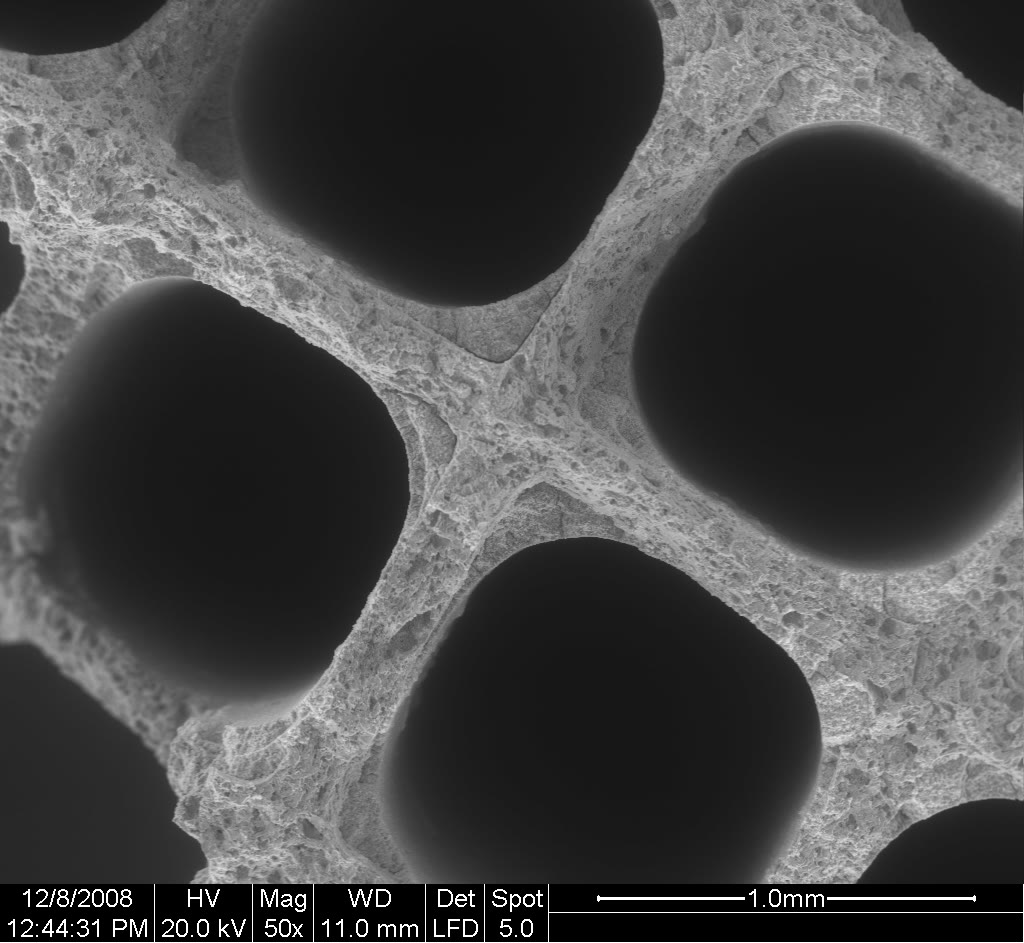
\includegraphics[width=0.48\linewidth]{images/book4/converter-sem.jpg}

{\small A colmeia cerâmica de um conversor catalítico vista ao microscópio
eletrônico de varredura (barra de escala de \qty{1.0}{mm}): canais quadrados separados
por paredes porosas finas, que carregam o revestimento de óxido e suas partículas metálicas.}
\end{omfigure}

\section{Adsorção}

\begin{definition}[Adsorção]\label{def:b3:surfaces-catalysis:adsorption}
A \emph{adsorção}\index{adsorcao@adsorção} é o acúmulo de moléculas de um gás ou de um
soluto na superfície de um sólido ou de um líquido. A molécula que se adsorve é o
\emph{adsorbato}\index{adsorbato}, o sólido é o \emph{adsorvente}\index{adsorvente};
o processo inverso é a \emph{dessorção}\index{dessorcao@dessorção}.
\end{definition}

\begin{definition}[Fisissorção, quimissorção]\label{def:b3:surfaces-catalysis:physi-chemi}
A \emph{fisissorção}\index{fisissorcao@fisissorção} é a \omterm{def:b3:surfaces-catalysis:adsorption}{adsorção} por forças de van der Waals,
com entalpias de \omterm{def:b3:surfaces-catalysis:adsorption}{adsorção} de algumas dezenas de quilojoules por mol no máximo,
comparáveis às entalpias de condensação, e sem alteração da molécula. A
\emph{quimissorção}\index{quimissorcao@quimissorção} forma ligações químicas com a superfície,
com entalpias de cerca de 40 a várias centenas de quilojoules por mol; ela pode
romper a molécula (quimissorção dissociativa) e se limita a uma única camada.
\end{definition}

\begin{omfigure}
\begin{tikzpicture}[font=\small, >=Stealth, x=1cm, y=1cm]
  \draw[->] (0,-2.6) -- (0,1.8) node[anchor=south] {energia};
  \draw[->] (0,0) -- (8.0,0) node[anchor=south east] {distância à superfície};
  \draw[omDef, thick] plot[smooth, tension=0.7] coordinates {(1.6,1.6) (2.2,-0.25) (2.8,-0.62) (3.6,-0.35) (5.0,-0.08) (7.5,0)};
  \draw[omThm, thick] plot[smooth, tension=0.6] coordinates {(0.45,1.6) (0.8,-1.2) (1.2,-2.2) (1.7,-1.6) (2.35,-0.15) (2.9,0.9) (3.5,1.5)};
  \node[omDef, anchor=north west, font=\scriptsize] at (3.4,-0.4) {\ce{H2} fisissorvido (precursor)};
  \node[omThm, anchor=west, font=\scriptsize] at (1.75,-1.9) {2 H quimissorvidos};
  \node[omThm, anchor=west, font=\scriptsize, align=left] at (3.55,1.45) {em direção a $\mathrm{H} + \mathrm{H}$\\ longe da superfície};
  \fill (2.3,-0.2) circle (1.5pt);
  \node[font=\scriptsize] (cr) at (1.25,0.55) {encontro};
  \draw[black!60] (cr.south east) -- (2.27,-0.15);
\end{tikzpicture}

{\small Energia potencial de uma molécula de hidrogênio que se aproxima de uma
superfície metálica (esquema). A molécula cai primeiro no poço raso da \omterm{def:b3:surfaces-catalysis:physi-chemi}{fisissorção};
onde essa curva cruza a curva de dois átomos de H ligados separadamente, ela pode se
dissociar e passar ao poço profundo da \omterm{def:b3:surfaces-catalysis:physi-chemi}{quimissorção}. Se o cruzamento fica acima de
zero, a \omterm{def:b3:surfaces-catalysis:physi-chemi}{quimissorção} dissociativa é ativada.}
\end{omfigure}

As superfícies das partículas metálicas expõem sobretudo as faces mais densas da
rede CFC, (111) e (100). Nelas, um \omterm{def:b3:surfaces-catalysis:adsorption}{adsorbato} pode ficar sobre um átomo
(posição de topo), entre dois (ponte) ou em uma cavidade entre três ou quatro, e a
energia de ligação difere de um sítio para outro.

\begin{omfigure}
\begin{tikzpicture}[font=\scriptsize]
  % fcc(111): hexagonal layer, spacing 0.6 cm
  \foreach \i in {0,...,5}{\foreach \j in {0,...,4}{
    \shade[ball color=black!25] ({0.6*\i+0.3*\j},{0.52*\j}) circle (0.29);}}
  \fill[omThm] (1.2+0.3*1,0.52) circle (0.07);
  \fill[omDef] ({0.6*2+0.3*2+0.3},{0.52*2}) circle (0.07);
  \fill[black] ({0.6*3+0.3*2+0.3},{0.52*2+0.17}) circle (0.07);
  \fill[black!60!green] ({0.6*1+0.3*3+0.3},{0.52*3-0.17}) circle (0.07);
  \node[anchor=north] at (2.1,-0.45) {CFC(111)};
  % fcc(100): square layer
  \begin{scope}[xshift=5.6cm]
  \foreach \i in {0,...,4}{\foreach \j in {0,...,4}{
    \shade[ball color=black!25] ({0.6*\i},{0.6*\j}) circle (0.29);}}
  \fill[omThm] (1.2,1.2) circle (0.07);
  \fill[omDef] (1.5,1.8) circle (0.07);
  \fill[black] (2.1,0.9) circle (0.07);
  \node[anchor=north] at (1.2,-0.45) {CFC(100)};
  \end{scope}
  \node[anchor=west, align=left] at (9.0,1.6) {\textcolor{omThm}{$\bullet$} topo\\ \textcolor{omDef}{$\bullet$} ponte\\
    $\bullet$ cavidade (3 ou 4 vizinhos)\\ \textcolor{black!60!green}{$\bullet$} segunda cavidade ternária (111)};
\end{tikzpicture}

{\small Vistas de cima das duas faces mais densas de um metal cúbico de faces
centradas, com os sítios de \omterm{def:b3:surfaces-catalysis:adsorption}{adsorção}: no topo de um átomo, em ponte entre dois e nas
cavidades entre três átomos em (111) (de dois tipos, acima ou não de um átomo da
segunda camada) ou quatro átomos em (100).}
\end{omfigure}

\begin{definition}[Grau de recobrimento, monocamada]\label{def:b3:surfaces-catalysis:coverage}
O \emph{grau de recobrimento}\index{grau de recobrimento} $\theta$ de uma superfície é a
fração de seus sítios de \omterm{def:b3:surfaces-catalysis:adsorption}{adsorção} que estão ocupados. Uma
\emph{monocamada}\index{monocamada} é uma única camada completa de \omterm{def:b3:surfaces-catalysis:adsorption}{adsorbato}, $\theta = 1$.
\end{definition}

\section{Isotermas}

\begin{theorem}[Isoterma de Langmuir]\label{thm:b3:surfaces-catalysis:langmuir}
Se uma superfície tem sítios idênticos e independentes, cada um comportando uma
molécula, o \omterm{def:b3:surfaces-catalysis:coverage}{grau de recobrimento} em equilíbrio com um gás à pressão $p$ é
\[
  \theta = \frac{Kp}{1 + Kp},
\]
onde $K$, a constante de equilíbrio de \omterm{def:b3:surfaces-catalysis:adsorption}{adsorção}, depende apenas da temperatura.
Esta é a \emph{isoterma de Langmuir}\index{isoterma de Langmuir}.
\end{theorem}

\begin{proof}
Demonstração cinética. As moléculas se adsorvem nos sítios livres com a velocidade
$k_ap(1 - \theta)N$ ($N$ sítios) e se dessorvem com a velocidade $k_d\theta N$. No equilíbrio,
as duas são iguais: $\theta/(1 - \theta)
= (k_a/k_d)p$, que se rearranja no resultado com $K = k_a/k_d$.

Demonstração estatística. $M$ moléculas sobre $N$ sítios podem ser dispostas de $N!/(M!(N - M)!)$
maneiras, cada molécula adsorvida tendo uma função de partição interna $q_{\mathrm s}$
(suas vibrações contra a superfície e sua energia de ligação). Com a fórmula de
Stirling, o potencial químico das moléculas adsorvidas é $\mu_{\mathrm s} = -kT\ln\bigl(q_{\mathrm s}\frac{1 - \theta}{\theta}\bigr)$;
o do gás ideal é $\mu_{\mathrm g} = \mu_{\mathrm g}^\circ + kT\ln(p/p^\circ)$. O equilíbrio, $\mu_{\mathrm s} = \mu_{\mathrm g}$, dá
$\theta/(1 - \theta) = q_{\mathrm s}\eu^{\mu_{\mathrm g}^\circ/kT}p/p^\circ$: a mesma lei, com $K$ escrita em termos de
funções de partição.
\end{proof}

A baixa pressão, $\theta \approx Kp$ (regime de Henry); a alta pressão, $\theta \to 1$. O \omterm{def:b3:surfaces-catalysis:coverage}{grau
de recobrimento} vale um meio em $p = 1/K$.

\begin{proposition}[Adsorção dissociativa]\label{prop:b3:surfaces-catalysis:dissociative}
Para um gás diatômico que se dissocia sobre dois sítios, $\mathrm{H_2} + 2\,{*} \to 2\,\mathrm{H}{*}$ (${*}$: um sítio livre),
\[
  \theta = \frac{(Kp)^{1/2}}{1 + (Kp)^{1/2}},
\]
de modo que $\theta \propto \sqrt p$ a baixa pressão.
\end{proposition}

\begin{proof}
A \omterm{def:b3:surfaces-catalysis:adsorption}{adsorção} exige dois sítios livres, com a velocidade $k_ap(1 - \theta)^2$; a \omterm{def:b3:surfaces-catalysis:adsorption}{dessorção} exige
que dois átomos adsorvidos se recombinem, com a velocidade $k_d\theta^2$. A igualdade dá $\theta/(1 - \theta) =
(Kp)^{1/2}$.
\end{proof}

\begin{proposition}[Adsorção competitiva]\label{prop:b3:surfaces-catalysis:competitive}
Dois gases A e B que competem pelos mesmos sítios os recobrem com
\[
  \theta_{\mathrm A} = \frac{K_{\mathrm A}p_{\mathrm A}}{1 + K_{\mathrm A}p_{\mathrm A} + K_{\mathrm B}p_{\mathrm B}}, \qquad
  \theta_{\mathrm B} = \frac{K_{\mathrm B}p_{\mathrm B}}{1 + K_{\mathrm A}p_{\mathrm A} + K_{\mathrm B}p_{\mathrm B}} .
\]
\end{proposition}

\begin{proof}
Para cada gás, $k_{a,\mathrm A}p_{\mathrm A}(1 - \theta_{\mathrm A} - \theta_{\mathrm B}) = k_{d,\mathrm A}\theta_{\mathrm A}$, e o mesmo para B. Logo
$\theta_{\mathrm A} = K_{\mathrm A}p_{\mathrm A}\theta_\ast$ e $\theta_{\mathrm B} = K_{\mathrm B}p_{\mathrm B}\theta_\ast$, com $\theta_\ast = 1 - \theta_{\mathrm A} - \theta_{\mathrm B}$ a fração livre; somando,
$1 - \theta_\ast = \theta_\ast(K_{\mathrm A}p_{\mathrm A} + K_{\mathrm B}p_{\mathrm B})$.
\end{proof}

\begin{definition}[Entalpia isostérica de adsorção]\label{def:b3:surfaces-catalysis:isosteric}
A \emph{entalpia isostérica de adsorção}\index{entalpia isosterica de adsorcao@entalpia isostérica de adsorção}
$\Delta_{\mathrm{ads}}H$ é a entalpia molar de \omterm{def:b3:surfaces-catalysis:adsorption}{adsorção} a \omterm{def:b3:surfaces-catalysis:coverage}{grau de recobrimento} fixo,
obtida a partir das pressões que dão o mesmo recobrimento em temperaturas
diferentes.
\end{definition}

\begin{proposition}[Entalpia isostérica]\label{prop:b3:surfaces-catalysis:isosteric}
A recobrimento constante,
\[
  \Bigl(\frac{\partial\ln p}{\partial T}\Bigr)_\theta = -\frac{\Delta_{\mathrm{ads}}H}{RT^2} .
\]
\end{proposition}

\begin{proof}
A $\theta$ constante, $Kp$ é constante (para uma superfície de Langmuir; em geral, o mesmo
argumento vale com a constante de equilíbrio nesse recobrimento), logo $\ln p =
\text{const} - \ln K$. Pela equação de van 't Hoff, $\dd\ln K/\dd T = \Delta_{\mathrm{ads}}H/RT^2$ (com $K$
referida a uma pressão padrão).
\end{proof}

Como a \omterm{def:b3:surfaces-catalysis:adsorption}{adsorção} é exotérmica, temperaturas mais altas exigem pressões mais altas
para o mesmo recobrimento: as isotermas da figura baixam quando $T$ sobe.

\begin{theorem}[Isoterma BET]\label{thm:b3:surfaces-catalysis:bet}
Se as moléculas se adsorvem em camadas sucessivas, a primeira com uma constante de
ligação característica da superfície e as demais com o equilíbrio de condensação
do líquido, a quantidade adsorvida à pressão relativa $x = p/p^*$ ($p^*$: pressão de
vapor do \omterm{def:b3:surfaces-catalysis:adsorption}{adsorbato} líquido) é
\[
  \frac{v}{v_{\mathrm m}} = \frac{cx}{(1 - x)(1 - x + cx)},
\]
onde $v_{\mathrm m}$ é a quantidade em uma \omterm{def:b3:surfaces-catalysis:coverage}{monocamada} e $c$ uma constante ligada à
diferença entre as entalpias de \omterm{def:b3:surfaces-catalysis:adsorption}{adsorção} na primeira camada e de condensação.
Esta é a \emph{isoterma BET}\index{isoterma BET} (Brunauer, Emmett e Teller).
\end{theorem}

\begin{proof}
Seja $s_i$ a fração da superfície coberta por exatamente $i$ camadas. O balanço de
cada camada, como na demonstração de Langmuir, dá $s_1 = cxs_0$ e $s_i =
xs_{i-1}$ para $i \ge 2$, logo $s_i = cx^is_0$. A quantidade adsorvida é $v/v_{\mathrm m} =
\sum_iis_i/\sum_is_i$. Com $\sum_{i\ge1}x^i = x/(1 - x)$ e $\sum_{i\ge1}ix^i = x/(1 - x)^2$:
\[
  \frac{v}{v_{\mathrm m}} = \frac{cs_0\,x/(1 - x)^2}{s_0[1 + cx/(1 - x)]} = \frac{cx}{(1 - x)(1 - x + cx)} .
\]
\end{proof}

Rearranjada, $\dfrac{x}{v(1 - x)} = \dfrac{1}{v_{\mathrm m}c} + \dfrac{c - 1}{v_{\mathrm m}c}\,x$: uma reta cuja inclinação e
cujo intercepto dão $v_{\mathrm m}$ e $c$, em geral válida para $0.05 < x < 0.30$.

\begin{definition}[Área superficial específica]\label{def:b3:surfaces-catalysis:surface-area}
A \emph{área superficial específica}\index{area superficial especifica@área superficial específica} de um sólido é sua
área superficial por unidade de massa, incluindo as paredes de seus poros.
\end{definition}

\begin{method}[Área superficial específica a partir de uma isoterma de nitrogênio]\label{met:b3:surfaces-catalysis:bet-area}
\begin{enumerate}
  \item Desgaseifique a amostra sob vácuo, aquecendo-a; resfrie-a em nitrogênio
        líquido (\qty{77}{K}).
  \item Meça o volume de nitrogênio adsorvido (reduzido às condições padrão) a
        pressões relativas entre 0.05 e 0.30.
  \item Trace $x/(v(1 - x))$ em função de $x$; a partir da inclinação e do intercepto,
        $v_{\mathrm m} = 1/(\text{inclinação} + \text{intercepto})$ e $c = 1 + \text{inclinação}/\text{intercepto}$.
  \item Área $= n_{\mathrm m}N_Aa_{\mathrm m}$, com $n_{\mathrm m}$ a quantidade na \omterm{def:b3:surfaces-catalysis:coverage}{monocamada} e $a_{\mathrm m} = \qty{0.162}{nm^2}$
        a área convencional de uma molécula de nitrogênio adsorvida.
\end{enumerate}
\end{method}

\begin{omfigure}
\begin{tikzpicture}
\begin{axis}[name=la, width=0.31\linewidth, height=5.0cm, xmin=0, xmax=100, ymin=0, ymax=1.05,
  axis lines=left, xlabel={$p$ / kPa}, ylabel={$\theta$}, tick label style={font=\small},
  label style={font=\small}, title={\small Langmuir}]
\addplot[omDef, thick] table[x=p_kPa, y=T300] {figdata/out/bachelor-3-langmuir-bet-langmuir.dat};
\addplot[omThm, thick] table[x=p_kPa, y=T350] {figdata/out/bachelor-3-langmuir-bet-langmuir.dat};
\node[font=\scriptsize, omDef, anchor=south east] at (axis cs:98,0.92) {\qty{300}{K}};
\node[font=\scriptsize, omThm, anchor=north east] at (axis cs:98,0.45) {\qty{350}{K}};
\end{axis}
\begin{axis}[name=be, at={(la.east)}, anchor=west, xshift=1.9cm, width=0.31\linewidth, height=5.0cm,
  xmin=0, xmax=0.9, ymin=0, ymax=200, axis lines=left, xlabel={$p/p^*$},
  ylabel={$v$ / \unit{cm^3.g^{-1}}}, tick label style={font=\small}, label style={font=\small},
  title={\small BET}]
\addplot[black, thick] table[x=x, y=v] {figdata/out/bachelor-3-langmuir-bet-bet.dat};
\addplot[only marks, mark=*, mark size=1.4pt, omDef] table[x=x, y=v] {figdata/out/bachelor-3-langmuir-bet-data.dat};
\draw[black!40, dashed] (axis cs:0,45) -- (axis cs:0.9,45);
\node[font=\scriptsize, anchor=south east] at (axis cs:0.88,45) {$v_{\mathrm m}$};
\end{axis}
\begin{axis}[at={(be.east)}, anchor=west, xshift=2.1cm, width=0.31\linewidth, height=5.0cm,
  xmin=0, xmax=0.35, ymin=0, ymax=0.0085, axis lines=left, xlabel={$x = p/p^*$},
  ylabel={$x/(v(1 - x))$}, tick label style={font=\small}, label style={font=\small},
  scaled y ticks=false, yticklabel style={/pgf/number format/fixed, /pgf/number format/precision=3},
  title={\small gráfico BET}]
\addplot[black, thin] table[x=x, y=y] {figdata/out/bachelor-3-langmuir-bet-line.dat};
\addplot[only marks, mark=*, mark size=1.4pt, omDef] table[x=x, y=y] {figdata/out/bachelor-3-langmuir-bet-data.dat};
\end{axis}
\end{tikzpicture}

{\small À esquerda: \omterm{thm:b3:surfaces-catalysis:langmuir}{isotermas de Langmuir} de uma quimissorção-modelo ($\Delta_{\mathrm{ads}}H = \qty{-40}{kJ/mol}$) em
duas temperaturas. No meio: uma \omterm{thm:b3:surfaces-catalysis:bet}{isoterma BET} (modelo, $v_{\mathrm m} = \qty{45}{cm^3.g^{-1}}$, $c = 120$), com os
pontos do problema de fim de semana; as camadas se empilham e a quantidade diverge perto
de $p = p^*$, onde o gás se condensa. À direita: o gráfico BET linear dos mesmos pontos.}
\end{omfigure}

\section{Cinética das reações de superfície}

\begin{definition}[Mecanismos de Langmuir--Hinshelwood e de Eley--Rideal]\label{def:b3:surfaces-catalysis:mechanisms}
No \emph{mecanismo de Langmuir--Hinshelwood}\index{mecanismo de Langmuir--Hinshelwood}, os
dois reagentes estão adsorvidos e reagem na superfície; no \emph{mecanismo de
Eley--Rideal}\index{mecanismo de Eley--Rideal}, um reagente adsorvido reage com uma
molécula que chega da fase gasosa.
\end{definition}

\begin{proposition}[Velocidade de Langmuir--Hinshelwood]\label{prop:b3:surfaces-catalysis:lh-rate}
Se os equilíbrios de \omterm{def:b3:surfaces-catalysis:adsorption}{adsorção} são rápidos e a reação de superfície entre A e B
adsorvidos é a etapa determinante,
\[
  r = k\theta_{\mathrm A}\theta_{\mathrm B} = \frac{kK_{\mathrm A}p_{\mathrm A}K_{\mathrm B}p_{\mathrm B}}{(1 + K_{\mathrm A}p_{\mathrm A} + K_{\mathrm B}p_{\mathrm B})^2},
\]
que, a $p_{\mathrm B}$ fixa, é máxima quando $K_{\mathrm A}p_{\mathrm A} = 1 + K_{\mathrm B}p_{\mathrm B}$ e depois diminui à medida que A
expulsa B da superfície.
\end{proposition}

\begin{proof}
Os recobrimentos são os da \cref{prop:b3:surfaces-catalysis:competitive}. Com $u =
K_{\mathrm A}p_{\mathrm A}$ e $a = 1 + K_{\mathrm B}p_{\mathrm B}$, $r \propto u/(a + u)^2$, cuja derivada $(a - u)/(a + u)^3$ se anula em
$u = a$.
\end{proof}

\begin{proposition}[Velocidade de Eley--Rideal]\label{prop:b3:surfaces-catalysis:er-rate}
Se A adsorvido reage com B gasoso,
\[
  r = k\theta_{\mathrm A}p_{\mathrm B} = \frac{kK_{\mathrm A}p_{\mathrm A}p_{\mathrm B}}{1 + K_{\mathrm A}p_{\mathrm A}},
\]
que cresce com $p_{\mathrm A}$ até um patamar, sem máximo.
\end{proposition}

\begin{proof}
B não compete pelos sítios: $\theta_{\mathrm A}$ é o recobrimento de Langmuir de A sozinho, e a
velocidade é proporcional a ele e à frequência de colisão de B com a superfície,
proporcional a $p_{\mathrm B}$.
\end{proof}

\begin{method}[LH ou ER pela dependência com a pressão]\label{met:b3:surfaces-catalysis:mechanism-from-rate}
\begin{enumerate}
  \item Meça a velocidade em função da pressão de cada reagente, mantendo a outra
        fixa.
  \item Um máximo, seguido de queda (ordem negativa a alta pressão):
        Langmuir--Hinshelwood, com o reagente inibindo ao ocupar os sítios.
  \item Uma subida até um patamar em um reagente e primeira ordem no outro em todas
        as pressões: Eley--Rideal.
  \item Confirme com marcação isotópica ou espectroscopia de superfície; a maioria
        das reações catalíticas revela-se do tipo Langmuir--Hinshelwood.
\end{enumerate}
\end{method}

\begin{omfigure}
\begin{tikzpicture}
\begin{axis}[width=0.6\linewidth, height=5.4cm, xmin=0, xmax=10, ymin=0, ymax=0.3,
  axis lines=left, xlabel={$p_{\mathrm A}$ (reduzida)}, ylabel={velocidade (reduzida)},
  tick label style={font=\small}, label style={font=\small},
  legend style={font=\scriptsize, draw=none, at={(1.03,0.98)}, anchor=north west}, legend cell align=left]
\addplot[omDef!50, thick] table[x=pA, y=pB05] {figdata/out/bachelor-3-surface-rates.dat};
\addplot[omDef, thick] table[x=pA, y=pB1] {figdata/out/bachelor-3-surface-rates.dat};
\addplot[black, thick] table[x=pA, y=pB3] {figdata/out/bachelor-3-surface-rates.dat};
\addplot[omThm, thick, dashed] table[x=pA, y=ER] {figdata/out/bachelor-3-surface-rates.dat};
\legend{{LH, $p_{\mathrm B} = 0.5$}, {LH, $p_{\mathrm B} = 1$}, {LH, $p_{\mathrm B} = 3$}, {ER ($\times\frac14$)}}
\end{axis}
\end{tikzpicture}

{\small Velocidades de uma reação de superfície bimolecular em função da pressão de A
(unidades reduzidas, $K_{\mathrm A} = K_{\mathrm B} = 1$). Langmuir--Hinshelwood: cada curva tem máximo em $K_{\mathrm A}p_{\mathrm A} =
1 + K_{\mathrm B}p_{\mathrm B}$ e depois cai à medida que A desloca B. Eley--Rideal (tracejada, em escala): um patamar.}
\end{omfigure}

\begin{proposition}[Energia de ativação aparente]\label{prop:b3:surfaces-catalysis:apparent-ea}
Para uma reação de superfície unimolecular com \omterm{def:b3:surfaces-catalysis:adsorption}{adsorção} de Langmuir, $r = k\theta = kKp/(1 + Kp)$.
A baixo recobrimento, a energia de ativação medida é $E_{a,\mathrm{app}} = E_a + \Delta_{\mathrm{ads}}H$; a
alto recobrimento, é $E_a$.
\end{proposition}

\begin{proof}
A baixo recobrimento, $r \approx kKp$, logo $\dd\ln r/\dd T = \dd\ln k/\dd T + \dd\ln K/\dd T = (E_a + \Delta_{\mathrm{ads}}H)/RT^2$.
A alto recobrimento, $\theta \approx 1$ e $r \approx k$.
\end{proof}

Como $\Delta_{\mathrm{ads}}H < 0$, uma reação sobre uma superfície pouco recoberta parece mais fácil
do que sua barreira verdadeira: elevar a temperatura acelera a etapa de superfície,
mas esvazia a superfície.

\begin{definition}[Princípio de Sabatier, curva em vulcão]\label{def:b3:surfaces-catalysis:sabatier}
O \emph{princípio de Sabatier}\index{principio de Sabatier@princípio de Sabatier} afirma que o melhor
catalisador liga os reagentes nem fraco demais (eles não se adsorvem nem são
ativados) nem forte demais (os produtos não saem e bloqueiam os sítios). Uma
\emph{curva em vulcão}\index{curva em vulcao@curva em vulcão} da atividade de uma série de
catalisadores em função de uma energia de ligação tem um máximo em uma ligação intermediária.
\end{definition}

\begin{omfigure}
\begin{tikzpicture}[font=\small, >=Stealth]
  \draw[->] (0,0) -- (7.2,0) node[anchor=north east] {força de ligação do adsorbato};
  \draw[->] (0,0) -- (0,3.6) node[anchor=south] {atividade};
  \draw[omDef, very thick] (0.4,0.3) -- (3.4,3.0) -- (6.6,0.4);
  \node[anchor=south, align=center, font=\scriptsize] at (1.35,2.0) {liga fraco demais:\\ reagentes não\\ ativados};
  \node[anchor=south, align=center, font=\scriptsize] at (5.9,2.0) {liga forte demais:\\ produtos bloqueiam\\ os sítios};
  \node[anchor=south, font=\scriptsize] at (3.4,3.05) {melhor catalisador};
\end{tikzpicture}

{\small Uma \omterm{def:b3:surfaces-catalysis:sabatier}{curva em vulcão} (qualitativa): a atividade de uma série de catalisadores
em função da força com que eles ligam um intermediário-chave.}
\end{omfigure}

\section{Catalisadores industriais}

\begin{definition}[Concepção de catalisadores]\label{def:b3:surfaces-catalysis:catalyst-design}
Um \emph{suporte de catalisador}\index{suporte de catalisador} é um sólido poroso de grande
área (alumina, sílica, carbono) que carrega pequenas partículas da fase ativa. Um
\emph{promotor}\index{promotor} é um aditivo, inativo sozinho, que aumenta a
atividade, a seletividade ou a estabilidade. Um \emph{veneno de catalisador}\index{veneno de catalisador}
é uma substância que se liga fortemente aos \omterm{def:b3:complex-kinetics:enzyme}{sítios ativos} e os bloqueia.
A \emph{dispersão metálica}\index{dispersao metalica@dispersão metálica} $D$ é a fração dos átomos de
metal que ficam na superfície. A \emph{sinterização}\index{sinterizacao@sinterização} é o
crescimento das partículas a alta temperatura, que diminui a dispersão.
\end{definition}

\begin{method}[Dispersão e tamanho de partícula a partir da quimissorção de hidrogênio]\label{met:b3:surfaces-catalysis:dispersion}
\begin{enumerate}
  \item Reduza o catalisador em hidrogênio, evacue e meça o volume de \ce{H2}
        quimissorvido (reduzido às condições padrão) sobre o metal; o suporte não
        adsorve nada.
  \item Suponha um átomo de H por átomo de metal de superfície: $D = n_{\ce{H}}/n_{\text{metal}}$.
  \item Para esferas de diâmetro $d$, $D = 6(v_{\mathrm{at}}/a_{\mathrm{at}})/d$, com $v_{\mathrm{at}}$ o volume por átomo no
        interior do sólido e $a_{\mathrm{at}}$ a área por átomo de superfície; logo $d = 6v_{\mathrm{at}}/(a_{\mathrm{at}}D)$.
\end{enumerate}
\end{method}

A síntese da amônia, $\ce{N2 + 3 H2 <=> 2 NH3}$, ocorre a cerca de 400 a \qty{500}{\celsius} e 100 a
\qty{300}{bar} sobre ferro promovido com óxido de potássio e alumina: a alumina impede a
\omterm{def:b3:surfaces-catalysis:catalyst-design}{sinterização} dos cristalitos de ferro, o potássio aumenta a atividade. A etapa
determinante é a \omterm{def:b3:surfaces-catalysis:physi-chemi}{quimissorção} dissociativa de \ce{N2}, cuja ligação tripla é a
mais difícil de romper. Cerca de 150 milhões de toneladas de nitrogênio por ano são
fixadas dessa maneira.
% ledger: nh3:world-2024
A oxidação de \ce{SO2} a \ce{SO3}, sobre óxido de vanádio(V) promovido com sulfato
de potássio, é a etapa-chave da fabricação do ácido sulfúrico.

O conversor de três vias dos motores a gasolina oxida o CO e os hidrocarbonetos e
reduz os óxidos de nitrogênio ao mesmo tempo, sobre platina e paládio (oxidação) e
ródio (redução do NO), dispersos em alumina com óxido de cério, que armazena e libera
oxigênio. Ele só funciona em uma janela estreita em torno da razão ar--combustível
estequiométrica: com excesso de ar, o NO não é reduzido; com excesso de combustível,
o CO não é oxidado; uma sonda de oxigênio no escapamento mantém o motor dentro da
janela. O chumbo da gasolina com chumbo envenena o metal, o que é uma das razões do
desaparecimento dessa gasolina. As zeólitas, aluminossilicatos cristalinos com poros
de tamanho molecular e sítios ácidos, craqueiam as grandes moléculas das frações
pesadas do petróleo em gasolina e só admitem as moléculas que cabem em seus canais.

\begin{omfigure}
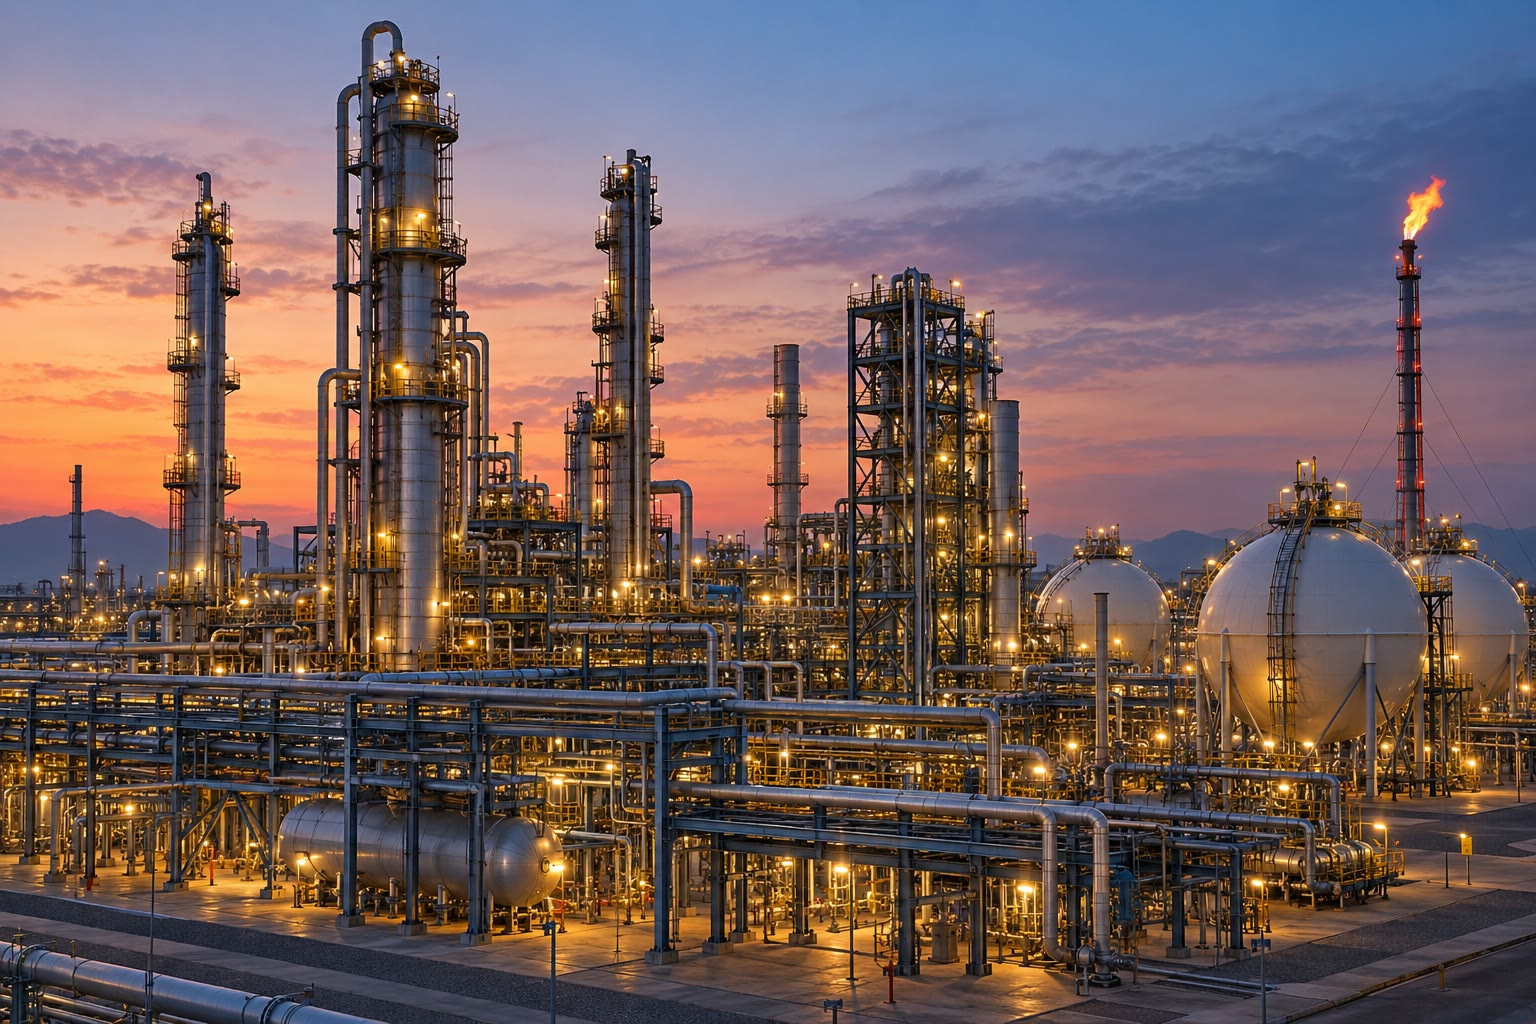
\includegraphics[width=0.6\linewidth]{images/book4/ai/b3-16-ammonia-plant.jpg}

{\small Uma usina de síntese de amônia. O reator em seu centro contém toneladas de
catalisador de ferro promovido; a maior parte da usina prepara o hidrogênio e recicla
o gás não convertido.}
\end{omfigure}

\section{Observar as superfícies}

\begin{definition}[Espectroscopia de dessorção térmica]\label{def:b3:surfaces-catalysis:tpd}
A \emph{espectroscopia de dessorção térmica}\index{espectroscopia de dessorcao termica@espectroscopia de dessorção térmica}
aquece a velocidade constante uma superfície que carrega um \omterm{def:b3:surfaces-catalysis:adsorption}{adsorbato} e registra o
gás dessorvido com um espectrômetro de massas; cada estado de ligação dá um pico,
cuja temperatura aumenta com sua energia de ativação de \omterm{def:b3:surfaces-catalysis:adsorption}{dessorção}.
\end{definition}

A posição de um pico de \omterm{def:b3:surfaces-catalysis:adsorption}{dessorção} dá a energia de \omterm{def:b3:surfaces-catalysis:adsorption}{dessorção} (para uma \omterm{def:b3:surfaces-catalysis:adsorption}{dessorção} de
primeira ordem, $E_d \approx RT_{\mathrm p}[\ln(\nu T_{\mathrm p}/\beta) - 3.64]$, com $\beta$ a velocidade de aquecimento e $\nu \approx \qty{e13}{s^{-1}}$,
admitido), e sua área, a quantidade adsorvida. A espectroscopia de fotoelétrons
excitados por raios X (XPS) mede as energias de ligação dos elétrons de caroço dos
átomos da superfície, que identificam os elementos e seus estados de oxidação nos
primeiros nanômetros. O microscópio de \omterm{def:b3:quantum-model-systems:tunnelling}{tunelamento} desloca uma ponta fina a alguns
décimos de nanômetro acima de uma superfície condutora; a corrente de \omterm{def:b3:quantum-model-systems:tunnelling}{tunelamento}
(\cref{ch:b3:quantum-model-systems}) cai cerca de uma ordem de grandeza a cada
\qty{0.1}{nm} de distância adicional, de modo que mantê-la constante durante a
varredura mapeia a superfície átomo por átomo.

\begin{inthelab}[Uma medida BET]
Cerca de \qty{0.2}{g} de amostra é pesado em um tubo de vidro com bulbo, desgaseificado
durante horas sob vácuo a 150 a \qty{300}{\celsius}, pesado de novo e montado no
instrumento, com o bulbo imerso em um dewar de nitrogênio líquido. O instrumento
admite nitrogênio em pequenas doses e mede a pressão de equilíbrio depois de cada
uma, deduzindo a quantidade adsorvida do balanço do gás; o volume morto do tubo é
medido com hélio, que não se adsorve.
\end{inthelab}

\begin{safety}{\ghs[0.7cm]{GHS06}\ghs[0.7cm]{GHS07}\ghs[0.7cm]{GHS08}\ghs[0.7cm]{GHS09}}
% ledger: ghs4:V2O5, ghs4:Ni
Os catalisadores metálicos reduzidos (níquel, paládio ou platina finamente divididos
sobre um suporte, recém-reduzidos em hidrogênio) podem inflamar-se em contato com o
ar: são manipulados sob gás inerte e passivados antes do armazenamento. O níquel é
um sensibilizante cutâneo e um suspeito cancerígeno; o óxido de vanádio(V) é tóxico
se inalado e se ingerido, e pode provocar câncer. Os pós de catalisador são pesados
em um recinto ventilado.
\end{safety}

\begin{history}[Langmuir e o catalisador da amônia]
Irving Langmuir, que trabalhava com lâmpadas elétricas em um laboratório
industrial, deduziu sua isoterma em 1916--1918 da ideia de que os gases adsorvidos
formam uma camada com a espessura de uma molécula, e recebeu o Prêmio Nobel de
Química de 1932 por sua química de superfícies. Alguns anos antes, Alwin Mittasch
havia organizado a busca de um catalisador prático para a amônia: milhares de
composições foram testadas em pequenos reatores de alta pressão antes que se
escolhesse o catalisador de ferro promovido, ainda em uso. Foi uma das primeiras
triagens sistemáticas de catalisadores.
\end{history}

\section{Exercícios}

\begin{exercise}[$\star$]\label{exo:b3:surfaces-catalysis:1}
Um gás recobre 40\,\% de uma superfície de Langmuir a \qty{2.0}{kPa}. Calcule $K$ e o
recobrimento a \qty{10}{kPa}.
\end{exercise}

\begin{exercise}[$\star$]\label{exo:b3:surfaces-catalysis:2}
Duas entalpias de \omterm{def:b3:surfaces-catalysis:adsorption}{adsorção} são medidas sobre um metal: $-20$ e \qty{-150}{kJ/mol}. Qual
é \omterm{def:b3:surfaces-catalysis:physi-chemi}{fisissorção}, qual é \omterm{def:b3:surfaces-catalysis:physi-chemi}{quimissorção}? Qual poderia ser dissociativa?
\end{exercise}

\begin{exercise}[$\star$]\label{exo:b3:surfaces-catalysis:3}
Conte, por átomo de superfície, os sítios de topo, de ponte e de cavidade de uma
face (100) e de uma face (111) de um metal CFC.
\end{exercise}

\begin{exercise}[$\star$]\label{exo:b3:surfaces-catalysis:4}
Um catalisador converte \qty{3.0e-6}{mol} de reagente por grama e por segundo e
carrega \qty{1.5e-5}{mol} de sítios de superfície por grama. Calcule a frequência de rotação.
\end{exercise}

\begin{exercise}[$\star\star$]\label{exo:b3:surfaces-catalysis:5}
O hidrogênio se adsorve de modo dissociativo com $\theta = 0.10$ a \qty{1.0}{kPa}. Calcule $\theta$ a \qty{4.0}{kPa}.
\end{exercise}

\begin{exercise}[$\star\star$]\label{exo:b3:surfaces-catalysis:6}
O CO ($K = \qty{10}{kPa^{-1}}$) e o \ce{O2} ($K = \qty{0.5}{kPa^{-1}}$, não dissociativo neste modelo simples)
competem pelos sítios de uma superfície de platina a 1.0 e a \qty{5.0}{kPa}. Calcule os
dois recobrimentos e comente a velocidade de oxidação do CO.
\end{exercise}

\begin{exercise}[$\star\star$]\label{exo:b3:surfaces-catalysis:7}
Um recobrimento atingido a \qty{1.0}{kPa} a \qty{300}{K} exige \qty{8.0}{kPa} a \qty{350}{K}.
Calcule a \omterm{def:b3:surfaces-catalysis:isosteric}{entalpia isostérica de adsorção}.
\end{exercise}

\begin{exercise}[$\star\star$]\label{exo:b3:surfaces-catalysis:8}
% ledger: sa:N2.am, const:Vm1, const:NA
Um carvão ativado tem $v_{\mathrm m} = \qty{120}{cm^3.g^{-1}}$ (condições padrão, 273.15 K e
\qty{101.325}{kPa}). Calcule sua área BET.
\end{exercise}

\begin{exercise}[$\star\star$]\label{exo:b3:surfaces-catalysis:9}
A velocidade de $\ce{2 CO + O2 -> 2 CO2}$ sobre platina sobe, passa por um máximo e cai quando
$p(\ce{CO})$ aumenta a $p(\ce{O2})$ fixa. Que mecanismo isso indica, e por que o CO
inibe a reação?
\end{exercise}

\begin{exercise}[$\star\star\star$]\label{exo:b3:surfaces-catalysis:10}
Uma reação de superfície tem energia de ativação verdadeira de \qty{100}{kJ/mol}; o
reagente tem $\Delta_{\mathrm{ads}}H = \qty{-60}{kJ/mol}$. Que energia de ativação se mede a baixo e a
alto recobrimento? Esboce $\ln r$ em função de $1/T$ em um intervalo amplo.
\end{exercise}

\begin{exercise}[$\star\star\star$]\label{exo:b3:surfaces-catalysis:11}
O enxofre se adsorve sobre um catalisador de níquel com recobrimento de 0.10 (átomos
de enxofre por Ni de superfície), cada átomo de enxofre bloqueando quatro sítios. Que
fração da atividade resta para uma reação que precisa de um sítio livre? E de dois
sítios livres adjacentes (suponha os sítios bloqueados distribuídos ao acaso)?
\end{exercise}

\begin{exercise}[$\star\star\star$]\label{exo:b3:surfaces-catalysis:12}
Para a síntese da amônia, três metais ligam o nitrogênio atômico com entalpias de
$-150$, $-250$ e \qty{-400}{kJ/mol} (dados do exercício). Usando o \omterm{def:b3:surfaces-catalysis:sabatier}{princípio de
Sabatier}, qual é provavelmente o melhor catalisador, e o que limita os outros dois?
\end{exercise}

\section{Problema: Medindo um catalisador}

\begin{problem}[{Problema de fim de semana --- medindo um catalisador: a área BET de
um catalisador de platina suportada, sua dispersão metálica e o tamanho de suas
partículas pela quimissorção de hidrogênio, e a frequência de rotação de uma hidrogenação}]
\label{pb:b3:surfaces-catalysis:1}
% ledger: sa:N2.am, lat:Pt, aw:Pt, const:Vm1, const:NA
Um catalisador contém 1.00\,\% em massa de platina sobre alumina. Dados do problema:
isoterma de nitrogênio a \qty{77}{K} (volumes em condições padrão, 273.15 K e
\qty{101.325}{kPa}, por grama):
\begin{center}\small
\begin{tabular}{lcccccc}
\hline
$x = p/p^*$ & 0.05 & 0.10 & 0.15 & 0.20 & 0.25 & 0.30 \\
$v$ / \unit{cm^3.g^{-1}} & 41.2 & 46.1 & 51.1 & 54.1 & 58.9 & 62.9 \\ \hline
\end{tabular}
\end{center}
\ce{H2} quimissorvido sobre a platina: \qty{0.205}{cm^3} por grama de catalisador. Uma
hidrogenação ocorre a \qty{2.0e-5}{mol} por grama de catalisador por segundo. Platina: $M = \qty{195.08}{g/mol}$, cfc,
$a = \qty{392.3}{pm}$; volume molar de um gás nas condições padrão \qty{22414}{cm^3/mol};
$a_{\mathrm m}(\ce{N2}) = \qty{0.162}{nm^2}$.

\medskip\noindent\textbf{Parte I --- O gráfico BET.}
\begin{enumerate}
  \item Por que a isoterma é medida a \qty{77}{K}?
  \item Por que se usam apenas pressões relativas entre 0.05 e 0.30?
  \item Calcule $x/(v(1 - x))$ para cada ponto.
  \item A reta de mínimos quadrados tem inclinação \num{0.02205} e intercepto \num{0.000180} (em
        \unit{g.cm^{-3}}). Deduza $v_{\mathrm m}$.
  \item Deduza $c$. O que significa um $c$ grande?
  \item Por que o intercepto é tão mal determinado, e isso importa para $v_{\mathrm m}$?
\end{enumerate}

\medskip\noindent\textbf{Parte II --- A área.}
\begin{enumerate}[resume]
  \item Calcule a quantidade de nitrogênio na \omterm{def:b3:surfaces-catalysis:coverage}{monocamada} por grama.
  \item Calcule a \omterm{def:b3:surfaces-catalysis:surface-area}{área superficial específica}.
  \item Que parte do sólido fornece quase toda essa área?
  \item Por que o método BET falha para sólidos microporosos como as zeólitas?
\end{enumerate}

\medskip\noindent\textbf{Parte III --- Dispersão e tamanho das partículas.}
\begin{enumerate}[resume]
  \item Calcule a quantidade de átomos de H quimissorvidos por grama.
  \item Calcule a quantidade de platina por grama.
  \item Deduza a dispersão.
  \item Calcule o volume por átomo de Pt no interior do sólido.
  \item A área por átomo de superfície, média sobre as faces (111), (100) e (110),
        é de \qty{0.0807}{nm^2}. Verifique o valor para (111), $\frac{\sqrt3}{4}a^2$.
  \item Mostre que, para esferas, $d = 6v_{\mathrm{at}}/(a_{\mathrm{at}}D)$.
  \item Calcule o diâmetro médio das partículas.
  \item Que hipóteses limitam esse resultado?
\end{enumerate}

\medskip\noindent\textbf{Parte IV --- Atividade.}
\begin{enumerate}[resume]
  \item Calcule a frequência de rotação por átomo de Pt de superfície.
  \item Calcule a velocidade por grama de platina.
  \item Se as partículas sinterizassem até \qty{10}{nm} com frequência de rotação
        constante, por que fator cairia a velocidade por grama?
  \item O que revelaria uma frequência de rotação que muda com o tamanho das partículas?
  \item Por que os catalisadores são comparados pela frequência de rotação, e não pela
        velocidade por grama?
  \item Enuncie o resultado: o diâmetro médio das partículas de platina.
\end{enumerate}
\end{problem}
